
%% bare_conf.tex
%% V1.4b
%% 2015/08/26
%% by Michael Shell
%% See:
%% http://www.michaelshell.org/
%% for current contact information.
%%
%% This is a skeleton file demonstrating the use of IEEEtran.cls
%% (requires IEEEtran.cls version 1.8b or later) with an IEEE
%% conference paper.
%%
%% Support sites:
%% http://www.michaelshell.org/tex/ieeetran/
%% http://www.ctan.org/pkg/ieeetran
%% and
%% http://www.ieee.org/

%%*************************************************************************
%% Legal Notice:
%% This code is offered as-is without any warranty either expressed or
%% implied; without even the implied warranty of MERCHANTABILITY or
%% FITNESS FOR A PARTICULAR PURPOSE! 
%% User assumes all risk.
%% In no event shall the IEEE or any contributor to this code be liable for
%% any damages or losses, including, but not limited to, incidental,
%% consequential, or any other damages, resulting from the use or misuse
%% of any information contained here.
%%
%% All comments are the opinions of their respective authors and are not
%% necessarily endorsed by the IEEE.
%%
%% This work is distributed under the LaTeX Project Public License (LPPL)
%% ( http://www.latex-project.org/ ) version 1.3, and may be freely used,
%% distributed and modified. A copy of the LPPL, version 1.3, is included
%% in the base LaTeX documentation of all distributions of LaTeX released
%% 2003/12/01 or later.
%% Retain all contribution notices and credits.
%% ** Modified files should be clearly indicated as such, including  **
%% ** renaming them and changing author support contact information. **
%%*************************************************************************


% *** Authors should verify (and, if needed, correct) their LaTeX system  ***
% *** with the testflow diagnostic prior to trusting their LaTeX platform ***
% *** with production work. The IEEE's font choices and paper sizes can   ***
% *** trigger bugs that do not appear when using other class files.       ***                          ***
% The testflow support page is at:
% http://www.michaelshell.org/tex/testflow/



\documentclass[conference]{IEEEtran}
% Some Computer Society conferences also require the compsoc mode option,
% but others use the standard conference format.
%
% If IEEEtran.cls has not been installed into the LaTeX system files,
% manually specify the path to it like:
% \documentclass[conference]{../sty/IEEEtran}





% Some very useful LaTeX packages include:
\usepackage{balance}  % to better equalize the last page
\usepackage{graphics} % for EPS, load graphicx instead
\usepackage[pdftex]{hyperref}
% \usepackage{url}      % llt: nicely formatted URLs
\usepackage{booktabs}
%\usepackage{ccicons}
\usepackage{todonotes}
\usepackage{booktabs}
\usepackage{multirow}
% allows for temporary adjustment of side margins
\usepackage{chngpage}
\usepackage{enumerate}
 % provides filler text
 \usepackage{lipsum}
\usepackage{listings}
\usepackage{color}
\usepackage{siunitx}                      % improved handling of physical quantities and units
\usepackage[tableposition = top]{caption} % improved handling of caption
\usepackage{hyperref}
\usepackage{url}


\definecolor{dkgreen}{rgb}{0,0.6,0}
\definecolor{gray}{rgb}{0.5,0.5,0.5}
\definecolor{mauve}{rgb}{0.58,0,0.82}

\lstset{frame=tb,
	language=Java,
	aboveskip=3mm,
	belowskip=3mm,
	showstringspaces=false,
	columns=flexible,
	basicstyle={\small\ttfamily},
	numbers=none,
	numberstyle=\tiny\color{gray},
	keywordstyle=\color{blue},
	commentstyle=\color{dkgreen},
	stringstyle=\color{mauve},
	breaklines=true,
	breakatwhitespace=true,
	tabsize=3
}

\newcommand{\tania}[1]{\textcolor{red}{{\it [Tania says: #1]}}}
\newcommand{\nora}[1]{\textcolor{purple}{{\it [Nora says: #1]}}}

% *** MISC UTILITY PACKAGES ***
%
%\usepackage{ifpdf}
% Heiko Oberdiek's ifpdf.sty is very useful if you need conditional
% compilation based on whether the output is pdf or dvi.
% usage:
% \ifpdf
%   % pdf code
% \else
%   % dvi code
% \fi
% The latest version of ifpdf.sty can be obtained from:
% http://www.ctan.org/pkg/ifpdf
% Also, note that IEEEtran.cls V1.7 and later provides a builtin
% \ifCLASSINFOpdf conditional that works the same way.
% When switching from latex to pdflatex and vice-versa, the compiler may
% have to be run twice to clear warning/error messages.






% *** CITATION PACKAGES ***
%
%\usepackage{cite}
% cite.sty was written by Donald Arseneau
% V1.6 and later of IEEEtran pre-defines the format of the cite.sty package
% \cite{} output to follow that of the IEEE. Loading the cite package will
% result in citation numbers being automatically sorted and properly
% "compressed/ranged". e.g., [1], [9], [2], [7], [5], [6] without using
% cite.sty will become [1], [2], [5]--[7], [9] using cite.sty. cite.sty's
% \cite will automatically add leading space, if needed. Use cite.sty's
% noadjust option (cite.sty V3.8 and later) if you want to turn this off
% such as if a citation ever needs to be enclosed in parenthesis.
% cite.sty is already installed on most LaTeX systems. Be sure and use
% version 5.0 (2009-03-20) and later if using hyperref.sty.
% The latest version can be obtained at:
% http://www.ctan.org/pkg/cite
% The documentation is contained in the cite.sty file itself.






% *** GRAPHICS RELATED PACKAGES ***
%
\ifCLASSINFOpdf
  % \usepackage[pdftex]{graphicx}
  % declare the path(s) where your graphic files are
  % \graphicspath{{../pdf/}{../jpeg/}}
  % and their extensions so you won't have to specify these with
  % every instance of \includegraphics
  % \DeclareGraphicsExtensions{.pdf,.jpeg,.png}
\else
  % or other class option (dvipsone, dvipdf, if not using dvips). graphicx
  % will default to the driver specified in the system graphics.cfg if no
  % driver is specified.
  % \usepackage[dvips]{graphicx}
  % declare the path(s) where your graphic files are
  % \graphicspath{{../eps/}}
  % and their extensions so you won't have to specify these with
  % every instance of \includegraphics
  % \DeclareGraphicsExtensions{.eps}
\fi
% graphicx was written by David Carlisle and Sebastian Rahtz. It is
% required if you want graphics, photos, etc. graphicx.sty is already
% installed on most LaTeX systems. The latest version and documentation
% can be obtained at: 
% http://www.ctan.org/pkg/graphicx
% Another good source of documentation is "Using Imported Graphics in
% LaTeX2e" by Keith Reckdahl which can be found at:
% http://www.ctan.org/pkg/epslatex
%
% latex, and pdflatex in dvi mode, support graphics in encapsulated
% postscript (.eps) format. pdflatex in pdf mode supports graphics
% in .pdf, .jpeg, .png and .mps (metapost) formats. Users should ensure
% that all non-photo figures use a vector format (.eps, .pdf, .mps) and
% not a bitmapped formats (.jpeg, .png). The IEEE frowns on bitmapped formats
% which can result in "jaggedy"/blurry rendering of lines and letters as
% well as large increases in file sizes.
%
% You can find documentation about the pdfTeX application at:
% http://www.tug.org/applications/pdftex





% *** MATH PACKAGES ***
%
%\usepackage{amsmath}
% A popular package from the American Mathematical Society that provides
% many useful and powerful commands for dealing with mathematics.
%
% Note that the amsmath package sets \interdisplaylinepenalty to 10000
% thus preventing page breaks from occurring within multiline equations. Use:
%\interdisplaylinepenalty=2500
% after loading amsmath to restore such page breaks as IEEEtran.cls normally
% does. amsmath.sty is already installed on most LaTeX systems. The latest
% version and documentation can be obtained at:
% http://www.ctan.org/pkg/amsmath





% *** SPECIALIZED LIST PACKAGES ***
%
%\usepackage{algorithmic}
% algorithmic.sty was written by Peter Williams and Rogerio Brito.
% This package provides an algorithmic environment fo describing algorithms.
% You can use the algorithmic environment in-text or within a figure
% environment to provide for a floating algorithm. Do NOT use the algorithm
% floating environment provided by algorithm.sty (by the same authors) or
% algorithm2e.sty (by Christophe Fiorio) as the IEEE does not use dedicated
% algorithm float types and packages that provide these will not provide
% correct IEEE style captions. The latest version and documentation of
% algorithmic.sty can be obtained at:
% http://www.ctan.org/pkg/algorithms
% Also of interest may be the (relatively newer and more customizable)
% algorithmicx.sty package by Szasz Janos:
% http://www.ctan.org/pkg/algorithmicx




% *** ALIGNMENT PACKAGES ***
%
%\usepackage{array}
% Frank Mittelbach's and David Carlisle's array.sty patches and improves
% the standard LaTeX2e array and tabular environments to provide better
% appearance and additional user controls. As the default LaTeX2e table
% generation code is lacking to the point of almost being broken with
% respect to the quality of the end results, all users are strongly
% advised to use an enhanced (at the very least that provided by array.sty)
% set of table tools. array.sty is already installed on most systems. The
% latest version and documentation can be obtained at:
% http://www.ctan.org/pkg/array


% IEEEtran contains the IEEEeqnarray family of commands that can be used to
% generate multiline equations as well as matrices, tables, etc., of high
% quality.




% *** SUBFIGURE PACKAGES ***
%\ifCLASSOPTIONcompsoc
%  \usepackage[caption=false,font=normalsize,labelfont=sf,textfont=sf]{subfig}
%\else
%  \usepackage[caption=false,font=footnotesize]{subfig}
%\fi
% subfig.sty, written by Steven Douglas Cochran, is the modern replacement
% for subfigure.sty, the latter of which is no longer maintained and is
% incompatible with some LaTeX packages including fixltx2e. However,
% subfig.sty requires and automatically loads Axel Sommerfeldt's caption.sty
% which will override IEEEtran.cls' handling of captions and this will result
% in non-IEEE style figure/table captions. To prevent this problem, be sure
% and invoke subfig.sty's "caption=false" package option (available since
% subfig.sty version 1.3, 2005/06/28) as this is will preserve IEEEtran.cls
% handling of captions.
% Note that the Computer Society format requires a larger sans serif font
% than the serif footnote size font used in traditional IEEE formatting
% and thus the need to invoke different subfig.sty package options depending
% on whether compsoc mode has been enabled.
%
% The latest version and documentation of subfig.sty can be obtained at:
% http://www.ctan.org/pkg/subfig




% *** FLOAT PACKAGES ***
%
%\usepackage{fixltx2e}
% fixltx2e, the successor to the earlier fix2col.sty, was written by
% Frank Mittelbach and David Carlisle. This package corrects a few problems
% in the LaTeX2e kernel, the most notable of which is that in current
% LaTeX2e releases, the ordering of single and double column floats is not
% guaranteed to be preserved. Thus, an unpatched LaTeX2e can allow a
% single column figure to be placed prior to an earlier double column
% figure.
% Be aware that LaTeX2e kernels dated 2015 and later have fixltx2e.sty's
% corrections already built into the system in which case a warning will
% be issued if an attempt is made to load fixltx2e.sty as it is no longer
% needed.
% The latest version and documentation can be found at:
% http://www.ctan.org/pkg/fixltx2e


%\usepackage{stfloats}
% stfloats.sty was written by Sigitas Tolusis. This package gives LaTeX2e
% the ability to do double column floats at the bottom of the page as well
% as the top. (e.g., "\begin{figure*}[!b]" is not normally possible in
% LaTeX2e). It also provides a command:
%\fnbelowfloat
% to enable the placement of footnotes below bottom floats (the standard
% LaTeX2e kernel puts them above bottom floats). This is an invasive package
% which rewrites many portions of the LaTeX2e float routines. It may not work
% with other packages that modify the LaTeX2e float routines. The latest
% version and documentation can be obtained at:
% http://www.ctan.org/pkg/stfloats
% Do not use the stfloats baselinefloat ability as the IEEE does not allow
% \baselineskip to stretch. Authors submitting work to the IEEE should note
% that the IEEE rarely uses double column equations and that authors should try
% to avoid such use. Do not be tempted to use the cuted.sty or midfloat.sty
% packages (also by Sigitas Tolusis) as the IEEE does not format its papers in
% such ways.
% Do not attempt to use stfloats with fixltx2e as they are incompatible.
% Instead, use Morten Hogholm'a dblfloatfix which combines the features
% of both fixltx2e and stfloats:
%
% \usepackage{dblfloatfix}
% The latest version can be found at:
% http://www.ctan.org/pkg/dblfloatfix




% *** PDF, URL AND HYPERLINK PACKAGES ***
%
%\usepackage{url}
% url.sty was written by Donald Arseneau. It provides better support for
% handling and breaking URLs. url.sty is already installed on most LaTeX
% systems. The latest version and documentation can be obtained at:
% http://www.ctan.org/pkg/url
% Basically, \url{my_url_here}.




% *** Do not adjust lengths that control margins, column widths, etc. ***
% *** Do not use packages that alter fonts (such as pslatex).         ***
% There should be no need to do such things with IEEEtran.cls V1.6 and later.
% (Unless specifically asked to do so by the journal or conference you plan
% to submit to, of course. )


% correct bad hyphenation here
\hyphenation{op-tical net-works semi-conduc-tor}


\begin{document}
% The following command makes sure text doesn't go outside of the page limit
	\sloppy
	
%
% paper title
% Titles are generally capitalized except for words such as a, an, and, as,
% at, but, by, for, in, nor, of, on, or, the, to and up, which are usually
% not capitalized unless they are the first or last word of the title.
% Linebreaks \\ can be used within to get better formatting as desired.
% Do not put math or special symbols in the title.
\title{Climate Data Analysis with Amazon Web Services}


% author names and affiliations
% use a multiple column layout for up to three different
% affiliations
\author{\IEEEauthorblockN{Nora Huang\IEEEauthorrefmark{1},
		Maria Ferman\IEEEauthorrefmark{2}}
	\IEEEauthorblockA{Department of Computer Science, University of Victoria\\
		Victoria, BC, Canada\\
		Email: \IEEEauthorrefmark{1}norahuangsun@gmail.com,
		\IEEEauthorrefmark{2}tania.ferman@gmail.com}}
% conference papers do not typically use \thanks and this command
% is locked out in conference mode. If really needed, such as for
% the acknowledgment of grants, issue a \IEEEoverridecommandlockouts
% after \documentclass

% for over three affiliations, or if they all won't fit within the width
% of the page, use this alternative format:
% 
%\author{\IEEEauthorblockN{Michael Shell\IEEEauthorrefmark{1},
%Homer Simpson\IEEEauthorrefmark{2},
%James Kirk\IEEEauthorrefmark{3}, 
%Montgomery Scott\IEEEauthorrefmark{3} and
%Eldon Tyrell\IEEEauthorrefmark{4}}
%\IEEEauthorblockA{\IEEEauthorrefmark{1}School of Electrical and Computer Engineering\\
%Georgia Institute of Technology,
%Atlanta, Georgia 30332--0250\\ Email: see http://www.michaelshell.org/contact.html}
%\IEEEauthorblockA{\IEEEauthorrefmark{2}Twentieth Century Fox, Springfield, USA\\
%Email: homer@thesimpsons.com}
%\IEEEauthorblockA{\IEEEauthorrefmark{3}Starfleet Academy, San Francisco, California 96678-2391\\
%Telephone: (800) 555--1212, Fax: (888) 555--1212}
%\IEEEauthorblockA{\IEEEauthorrefmark{4}Tyrell Inc., 123 Replicant Street, Los Angeles, California 90210--4321}}




% use for special paper notices
%\IEEEspecialpapernotice{(Invited Paper)}




% make the title area
\maketitle

% As a general rule, do not put math, special symbols or citations
% in the abstract
\begin{abstract}
Nowadays, it is extremely important to work with big datasets, and work with that large amount of data it is not always straightforward. For example, in the climate research it is more and more common to work with thousands of climate stations that describe the climate from a particular location. With this analysis, climate scientists can have an accurate understanding of the climate change. Specifically, scientists need to have the average of the data according to a range of time and location, in order to discover anomalies in the climate, thus they can find monthly anomalies base on periods of time. Besides, this calculation allows to analyze if the current year was colder or warmer, or if the temperature is higher or lower than the previous years. Therefore, scientists need to deal with the issue of analyze huge datasets. For this reason new technologies such as the MapReduce paradigm allows us to have large-scale data analysis. However, the MapReduce paradigm is not easy to code, thus systems like Amazon Web Services is using Hadoop framework, Hive, Pig and Hue for helping users. AWS allows to have an easier and faster analysis. In this project we present an evaluation of Amazon Web Services by using a large dataset of a climate department. 

\end{abstract}

% no keywords




% For peer review papers, you can put extra information on the cover
% page as needed:
% \ifCLASSOPTIONpeerreview
% \begin{center} \bfseries EDICS Category: 3-BBND \end{center}
% \fi
%
% For peerreview papers, this IEEEtran command inserts a page break and
% creates the second title. It will be ignored for other modes.
\IEEEpeerreviewmaketitle
%!TEX root = DMmidterm.tex

\label{sec:introduction}
\section{Introduction}

Nowadays the size of the dataset that people is using is increasing considerably. Besides, users need a swift analysis of the data. Therefore, finding new technologies that allow users to analyze big data in a fast way is extremely important. Now users need a platform that is more agile, and with which they can manipulate, distribute and storing the data, and at the same time be able to build efficient scalable applications

Amazon Web Services is a cloud service platform that allows users to have a high compute power, a large durable dataset storage, high performance databases, among other functionalities. AWS provides to the users a large amount of services that they can use together for building the applications that they need.

Therefore, users can manage their data in an accessible way. Users can integrate, import and export the data, manage Hadoop and built secure environments for the analysis of large datasets.   

%!TEX root = DMmidterm.tex

\label{sec:relatedWork}
\section{Related work}
This section we will provide background on the distributed system techniques and tools that will be used in the project.

\subsection{MapReduce}
Nowadays, we need processes that support a large amount of data, and in order to do that, we need a group of computers working together to process that large amount of data. However, there are several issues we need to solve in order to accomplish these processes. For example, how to distribute the data, how to deal with some parts of the process fail, such as some nodes stop working.

Besides, there are also a specify data set processing problems. This data set includes raw data such as crawled documents and web request logs, derived data such inverted indices, various representations of the graph structure of web documents, summaries of the number of pages crawled per host, the set of most frequent queries in a given day. 

MapReduce is a functional model with user-specified map and reduce operations. It provides simple and powerful interface that enables automatic parallelization and distribution of large-scale computations, combined with an implementation of this interface that achieves high performance on large clusters of commodity PCs.

Specifically, the MapReduce solution is divided in two sections written by the user: Map and Reduce. On the Map section, it will be taken an input pair with which will be producing a key/value pairs. In this section, the MapReduce process will classify the values with their corresponded keys. Then, these classified pairs will be passed to the second section, the Reduce function.

In the Reduce section, it will receive the previously classified pairs, then, in this section it will be merged together the key with their corresponded values, in order to create a smaller set of values. In other words, the reduce phase collect intermediate results in order to have an assemble final result. \cite{dean2008mapreduce}

\subsection{Hadoop Distributed File System}

Another solution for solving Big Data problems is Hadoop Distributed File System\cite{shvachko2010hadoop}. In which the system will create replicas of the Data and divide them between different nodes. In order to do this, Hadoop uses the MapReduce paradigm. The data can be distributed among hundreds or thousands of nodes, and use parallel computations for having a reliable and scalable system. Specifically, the block of data will be carried out in the MapReduce system, in order to accomplish the big data processing requirements.

The process used by Hadoop starts by breaking the Data into small sections, consecutively all these small blocks of data will be distributed among the clusters. The reason for doing that division is for allowing the MapReduce system to work in parallel, thus the process can solve the scalability issues in systems that require Big Data.

Due to in all Distributed systems the presence of failures is inevitable, the fault tolerance and fault compensation capabilities are well understood by the Hadoop system. The solution found by Hadoop Distributed File system (HDFS) consist in having multiple sections (blocks) of the data and send them to different servers in the Hadoop cluster. Therefore HDFS uses these divisions of workloads into different servers in order to have the benefit of Data locality, a critical property when systems requires large Datasets.

For the sake of having a system that always maintains availability in the presence of failures, HDSF replicates small blocks of data into different servers. 

\subsection{Pig}

Pig \cite{gates2009building} was developed by Yahoo to allow users to focus more on the analysis of the data, rather than worry to write MapReduce implementations. By using Pig in Hadoop users can load any kind of data format. In order to compile the programs Pig uses its own language named Pig Latin.

Pig will use as an input pig latin program, and it will divide the program into different sections that will be used as MapReduce jobs. Then, this job sections will be executed and coordinated in the Hadoop MapReduce environment. Therefore, all the pig programs will be loaded into the MapReduce job cluster.

By using the Hadoop engine, Pig can have a remarkable fault-tolerance and scalability properties. 
The first step is loading the data, Pig will use a pig latin program as an input, then a set of transformations will be carried out by ping in order to translate the data in sections of MapReduce tasks. Then, when all the process ends, the Pig results can be shown on the screen or stored in a file.
 
\subsection{Hive}

As a result of some of the issues of the MapReduce model such as the low level and the requirement of building custom program, Facebook developed a new component that allows to users to leverage the Hadoop platform.  Users with a background in SQL can easily use the Hive platform developed on top of Hadoop, because the queries are similar to SQL statements \cite{thusoo2009hive}.

Specifically, SQL queries will be broken into blocks using the Hive Service for being used in the MapReduce jobs and being executed in the Hadoop cluster. The language that Hive provides is named HiveQL which is base on the SQL language, and uses statements such as select, project, joint among others. 

One of the main components of Hive is the Hive Thrift Server that is used to execute the HiveQL statements. The Hive Thrift Server is a simple client API used for allowing the communication with the Hive server. 
  
\subsection{Hue}

Hue \cite{rasheed2013fedora} stands for Hadoop User Experience, and it is an open source graphical interface that allows users to have an easier HDFS ecosystem experience by using a web basic application. Hue is a functional and intuitive tool that allows users to execute Hive jobs among other services on the web. Besides, Hue provides to the user with an automatic visualization at the end of the process, and users can change that graph by using simple operations.

Hue \cite{b2016professionalhadoop} is an application that allows users to upload, download and delete files in HDFS. After a file is uploaded, Hue will automatically extract the file to use. Therefore, Hue allows users to make a faster analysis of the data and HDFS file management in the web interface. 









  

%!TEX root = DMmidterm.tex

\section{Project}
\label{sec:Project}

%\begin{figure*}[]
%	\begin{center}
%		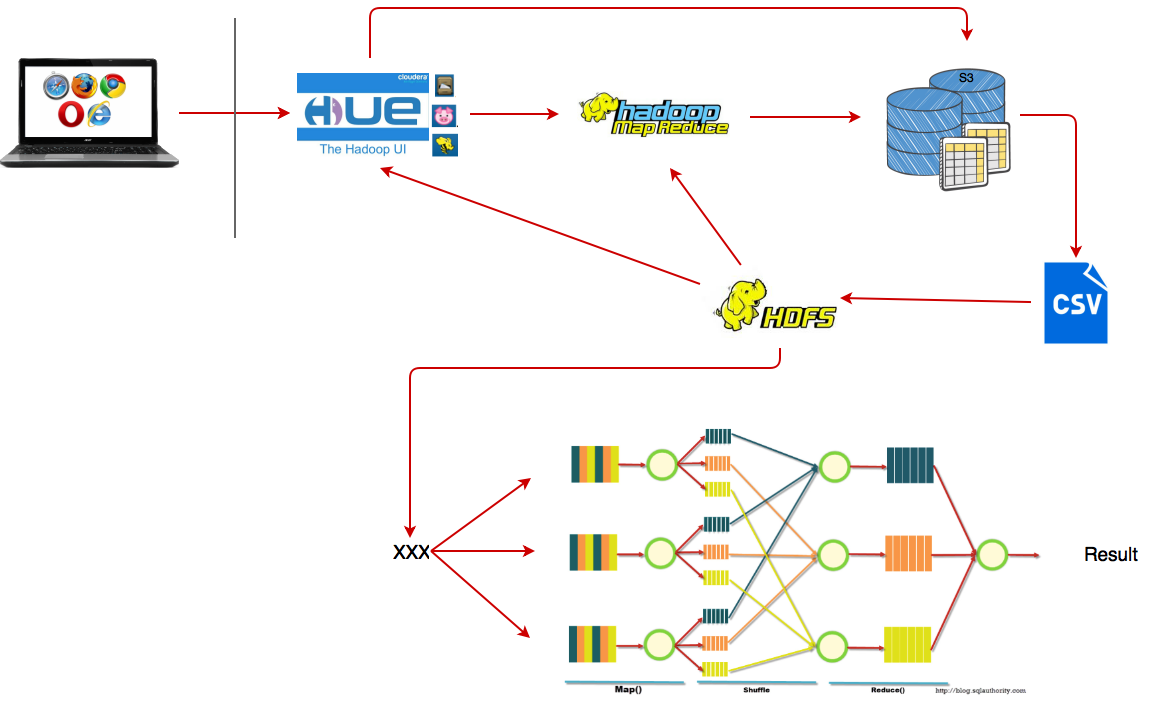
\includegraphics[width=2\columnwidth]{/Users/MariaFerman/Desktop/DC_FinalProject/images/Diagram}
%		\caption{Project Diagram}
%		\label{fig:dataDiagr}
%	\end{center}
%	\vspace{-10pt}
%\end{figure*}

%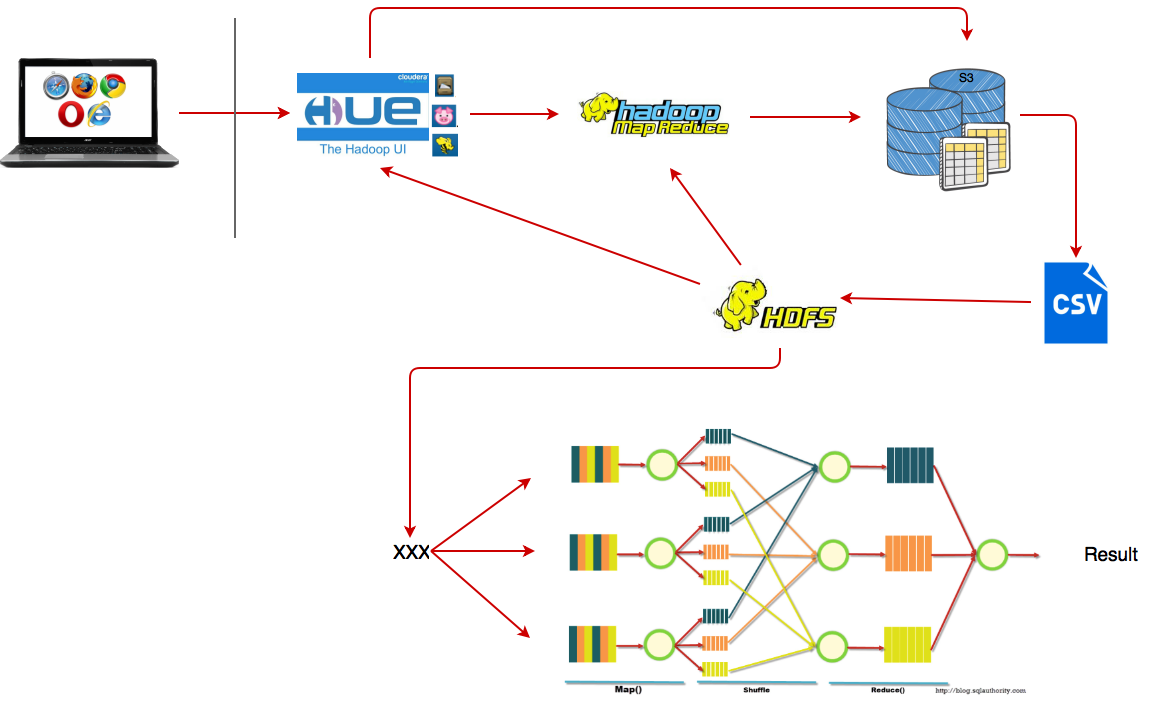
\includegraphics{/Users/MariaFerman/Desktop/DC_FinalProject/images/Diagram}


\subsection{ Dataset}
The dataset gathered for this project comes from the Pacific Climate Impacts Consortium (PCIC) of the University of Vic- toria. The dataset consist in a series of climate measurements that shows how the climate changes and varies over time. All the measurements were gathered at the same location in the Pacific and Yukon region of British Colombia, Canada. The dataset is divided by time and stations. The station is the exact location where the data were gathered. The dataset will allow us to understand the climate change among time and regions (stations). The resulting analysis of the dataset might help for trend analysis and climate change researches. This information can be used as an input for more complex climate models in order to have accurate climate predictions.


\subsection{Scripts}
The project has two main customised scripts for the Hive and Pig process. The first script is for getting the data and the second is for storing and computing the average of the data.

Pig script: This script has several crucial sections. The first one is when the data is extracted from the original CSV file. In the ”raw logs” variable it will be loaded the weblogs into a sequence of tuples.

\begin{lstlisting}
raw_logs =
  LOAD 's3://ds562finalproject/PacificClimate/
  2014_2015_MinTemp/' 
  USING TextLoader AS (line:chararray);
\end{lstlisting}

The second part of the script is for getting the information into the columns ''one\_day\_ precipitation'' for the percentage of precipitation, ''max\_temp'' for the maximum temperature and ''min\_temp'' for the minimum temperature for that specific day. Specifically, it will convert each weblog string into a structure with the above-mentioned columns.

\begin{lstlisting}
logs_base =
  FOREACH  raw_logs
  GENERATE
   FLATTEN (   	 
      EXTRACT(
        line, '^(\\d{4}-\\d{2})-\\d{2} \\d{2}:\\d{2}:\\d{2}, (\\S+), (\\S+), (\\S+)') )
    AS (
      date: chararray, one_day_precipitation: chararray, max_temp: chararray, min_temp: chararray )
\end{lstlisting}

On the next section, the data will be filter in order to separate the dates that have a non-null value. After that, the data will be grouped by the date field.  

\begin{lstlisting}
logs_no_null = FILTER logs_base BY date is not null; 
logs_group = GROUP logs_no_null BY date;
\end{lstlisting}

Finally, the last section of the script will compute the aver- age for the percentage of precipitation, maximum temperature and the minimum temperature. The last row is when the Hadoop file is created, this file will be used in the next section for visualizing the data.

\begin{lstlisting}
logs_avg = 
	FOREACH  logs_group
    GENERATE
      group,
      AVG(logs_no_null.one_day_precipitation),
      AVG(logs_no_null.max_temp),
      AVG(logs_no_null.min_temp);
      store logs_avg into '/user/NoraHuang/ds562’;
\end{lstlisting}

{Hive script}
This script uses sql command for selecting the data from the Hadoop Distributed File System. The script only select the require information for doing the posterior computations for analyzing of the data.

\begin{lstlisting}
SELECT ds562.time, ds562.one_day_precipitation, ds562.max_temp, ds562.min_temp 
FROM ds562
\end{lstlisting}

\subsection{Implementation}
We setup a EMR cluster on Amazon Web Service. The clus- ter consists of 3 nodes, 1 master and 2 core(workers servers). All nodes are running Lastest Ubuntu as its operating system while installed Hadoop, Hue, Hive and Pig by default. Hue is stalled on master node while the other 3 are architectures involved both master and core nodes. So we do not need to do extra configuration or application installation for our data analysis. The raw climate data are uploaded onto S3. And all output and logs are also stored in S3. The archtecure of the system are shown in fig1 and fig 2. fig1 shows the data process path of Pig while fig2 shows the data process path of Hive. We use Pig to load raw data from S3, and then caculate the average values of each columns and stored them in HDFS format. After the processed data are in HDFS, we can use Hive which provides SQL executor to access the data. Hue is a web page that providing interface for Pig and Hive.

%\begin{figure}[H]
\begin{figure*}[H]
	\begin{center}
		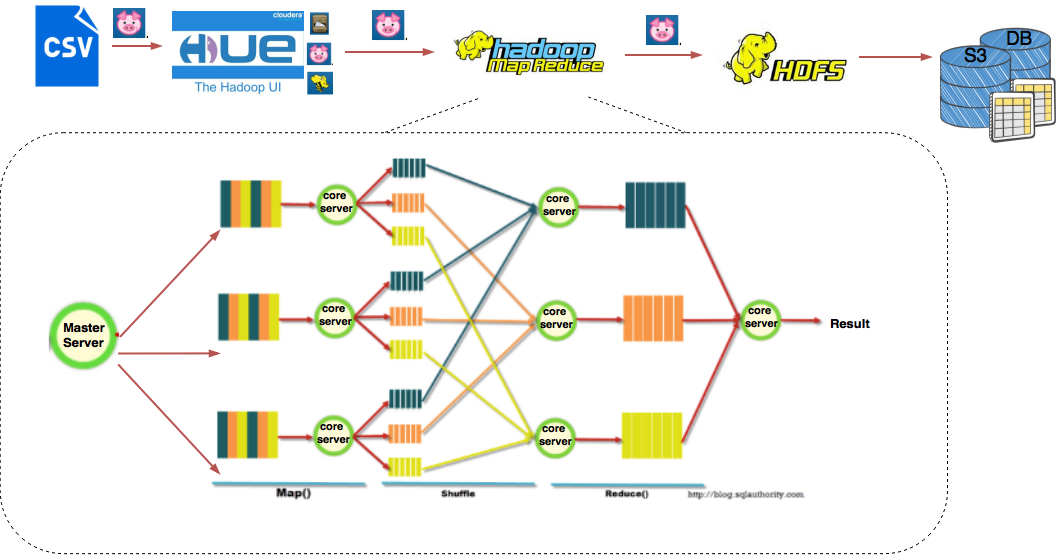
\includegraphics[width=2\columnwidth]{/Users/MariaFerman/Desktop/FinalReport/images/pigDiagram}
		\caption{Pig Diagram: shows the data process path of Pig}
		\label{fig:dataDiagr1}
	\end{center}
	\vspace{-10pt}
%\end{figure}
\end{figure*}

%\begin{figure}[H]
%\begin{figure*}[H]
	%\begin{center}
		%\includegraphics[width=2\columnwidth]{/Users/MariaFerman/Desktop/DC_FinalProject/images/HiveDiagram-2}
		%\caption{Hive Diagram}
		%\label{fig:dataDiagr2}
	%\end{center}
	%\vspace{-10pt}
%\end{figure}
%\end{figure*}

%\begin{figure}[H]
\begin{figure*}[H]
	\begin{center}
		\includegraphics[width=2\columnwidth]{/Users/MariaFerman/Desktop/FinalReport/images/HiveDiagram-2}
		\caption{Hive Diagram: shows the data process path of Hive.}
		\label{fig:dataDiagr3}
	\end{center}
	\vspace{-10pt}
%\end{figure}
\end{figure*}
%%!TEX root = DMmidterm.tex


\section{Project implementation}
\label{sec:projectImplementation}
In this section we present our implementation of the project in three phases. Dataset, Algorithm training, and Validation and analysis. 

\subsection{Phase I: Dataset}
\label{sec:dataset}
To add ...

%Pre-Defined Attributes


\subsection{Phase II: Algorithm Training}
\label{sec:training}

Pig To add ...
\begin{figure}[h!]
	\begin{center}
		\includegraphics[width=1\columnwidth]{/Users/MariaFerman/Desktop/DC_FinalProject/images/PigDiagram}
		\caption{Pig Diagram}
		\label{fig:dataDiagr}
	\end{center}
	\vspace{-10pt}
\end{figure}

Hive To add ...
\begin{figure}[h!]
	\begin{center}
		\includegraphics[width=1\columnwidth]{/Users/MariaFerman/Desktop/DC_FinalProject/images/HiveDiagram-2}
		\caption{Hive Diagram}
		\label{fig:dataDiagr}
	\end{center}
	\vspace{-10pt}
\end{figure}
(change subtitle to script?) 

%!TEX root = DMmidterm.tex


\section{Evaluation}
\label{sec:evaluation}
\subsection{Qualitatively}
\subsubsection*{Easy to Use}
You can launch an Amazon EMR cluster in minutes. You dont need to worry about node provisioning, cluster setup, Hadoop configuration, or cluster tuning. Amazon EMR takes care of these tasks so you can focus on analysis.

\subsubsection*{Predictable cost}
Amazon EMR pricing is simple and predictable: You pay an hourly rate for every instance hour you use. You can launch a 10-node Hadoop cluster for as little as \$0.15 per hour. Because Amazon EMR has native support for Amazon EC2 Spot and Reserved Instances, you can also save 50-80\% on the cost of the underlying instances.

\subsubsection*{Elastic}
With Amazon EMR, you can provision one, hun- dreds, or thousands of compute instances to process data at any scale. You can easily increase or decrease the number of instances and you only pay for what you use.

\subsubsection*{Reliable}
You can spend less time tuning and monitoring your cluster. Amazon EMR has tuned Hadoop for the cloud; it also monitors your cluster retrying failed tasks and automat- ically replacing poorly performing instances.

\subsubsection*{Flexible}
You have complete control over your cluster. You have root access to every instance, you can easily install additional applications, and you can customize every cluster. Amazon EMR also supports multiple Hadoop distributions and applications.

You can enjoy lots of features and benefits when you are using AWS EMR, however, graphical interface provided by Hue is limit, there are only several simple charts that it can display base on your data. And it is not user configurable. If you want a new chart type, you may need to change the source code of Hue. The good thing is that Hue is an open source project which you can access it source code and contribute on it easily.

%!!!!!!!!!!
\subsection{Quantitatively}
This section provides some pricing statistic and performance measurement on AWS EMR.

\subsubsection*{Pricing}
In our project the data is no more than 1GB. And we use 3 m3.xlarge nodes in our cluster each of which cost \$0.336 per hour. 
The detail of pricing can be found in Table~\ref{table1} and Table~\ref{table2}

\subsubsection*{Performance}
Since Pig is the most time consuming process in our data analysis, we only evaluate processing time of Pig. Hive take almost no time when access the processed data by Pig. We configure 1 m3.xlarge as master and 2 m3.xlarge as core. And execute the Pig Script on 1 year, 3 years, 5 years and 10 years data. 
Table~\ref{table3} demonstrate our measurement.


\begin{table}[]
\centering
\caption{S3 Storage Pricing}\label{table1}
\begin{tabular}{|l|l|l|l|}
\hline
/month       & \begin{tabular}[c]{@{}l@{}}Standard \\ Storage\\ per GB\end{tabular} & \begin{tabular}[c]{@{}l@{}}Standard- \\ Infrequent\\ Access \\ Storage †    \\ per GB\end{tabular} & \begin{tabular}[c]{@{}l@{}}Glacier \\ Storage\\ per GB\end{tabular} \\ \hline
First 1 TB   & \$0.0300                                                             & \$0.0125                                                                                           & \$0.007                                                             \\ \hline
Next 49 TB   & \$0.0295                                                             & \$0.0125                                                                                           & \$0.007                                                             \\ \hline
Next 450 TB  & \$0.0290                                                             & \$0.0125                                                                                           & \$0.007                                                             \\ \hline
Next 500 TB  & \$0.0285                                                             & \$0.0125                                                                                           & \$0.007                                                             \\ \hline
Next 4000 TB & \$0.0280                                                             & \$0.0125                                                                                           & \$0.007                                                             \\ \hline
Over 5000 TB & \$0.0275                                                             & \$0.0125                                                                                           & \$0.007                                                             \\ \hline
\end{tabular}
\end{table}


\begin{table}[]
\centering
\caption{Pricing for Amazon EMR and Amazon EC2
	General Purpose - Current Generation}\label{table2}
\begin{tabular}{|l|l|l|}
\hline
& \begin{tabular}[c]{@{}l@{}}Amazon EC2\\ per Hour\end{tabular} & \begin{tabular}[c]{@{}l@{}}Amazon Elastic MapReduce\\ per Hour\end{tabular} \\ \hline
m3.xlarge   & \$0.266                                                       & \$0.070                                                                     \\ \hline
m3.2xlarge  & \$0.532                                                       & \$0.140                                                                     \\ \hline
m4.large    & \$0.12                                                        & \$0.030                                                                     \\ \hline
m4.xlarge   & \$0.239                                                       & \$0.060                                                                     \\ \hline
m4.2xlarge  & \$0.479                                                       & \$0.120                                                                     \\ \hline
m4.4xlarge  & \$0.958                                                       & \$0.240                                                                     \\ \hline
m4.10xlarge & \$2.394                                                       & \$0.270                                                                     \\ \hline
\end{tabular}
\end{table}




\begin{table}[]
	\centering
	\caption{Pig Processing Time}
	\label{table3}
	\begin{tabular}{|l|l|}
		\hline
		\begin{tabular}[c]{@{}l@{}}Data Volume\\ year(s)\end{tabular} & \begin{tabular}[c]{@{}l@{}}Processing Time\\ ms\end{tabular} \\ \hline
		1                                                             & 37536                                                      \\ \hline
		3                                                             & 41908                                                      \\ \hline
		5                                                             & 42312                                                       \\ \hline
		10                                                            & 42054                                                      \\ \hline
	\end{tabular}
\end{table}

%!TEX root = DMmidterm.tex

\label{sec:conclusions}
\section{Conclusions}
To summarize, Amazon Web Services is a very efficient tool for the analysis of large datasets. By using AWS we were able to built a sophisticated and scalable application for the climate dataset that we have. We begin with the problem of how to analyze a big data in the climate field, and how to make some computations for getting the desired result, in this case having the average of the climate change of certain locations.

By using AWS we can experience how big data can be processed and managed, in order to have meaningful results. At the end of this project we can understand why many people and companies use AWS, due to it is very efficient and fast tool. After we understood how to configured  it and use the pig and hive process. We realized how simple and efficient is to use this infrastructure. The AWS takes care of the complex task of coding and manage the MapReduce algorithm, and we just need to focus on developing the Pig and Hive scripts.

At the end of this project, we were very satisfied about the results that we got. We were able to take a large data set and use a current and popular tool for solving our analysis needs. After devoting some time to understand this new technology for us, we are very satisfied about how a tool as the AWS can be used. Besides, we are confident that in the future we will be able to use similar technologies.



%!TEX root = DMmidterm.tex


\section{Future Work}
\label{sec:futureWork}
 We have spent most of our time dealing with the configuration of the AWS, and dealing with several issues with
the Pig and Hive script. Therefore, in our project there is room for improvement. One of the biggest enhancement of this paper will be the visualization part. Due to the reason above mentioned, we didn’t have time to create a customized visualization for the analysis of the climate dataset. Our current visualization is good enough for 1 or 2 years. However, when we need to visualize more years, all the data became obscure due to the large amount of results.


%









% An example of a floating figure using the graphicx package.
% Note that \label must occur AFTER (or within) \caption.
% For figures, \caption should occur after the \includegraphics.
% Note that IEEEtran v1.7 and later has special internal code that
% is designed to preserve the operation of \label within \caption
% even when the captionsoff option is in effect. However, because
% of issues like this, it may be the safest practice to put all your
% \label just after \caption rather than within \caption{}.
%
% Reminder: the "draftcls" or "draftclsnofoot", not "draft", class
% option should be used if it is desired that the figures are to be
% displayed while in draft mode.
%
%\begin{figure}[!t]
%\centering
%\includegraphics[width=2.5in]{myfigure}
% where an .eps filename suffix will be assumed under latex, 
% and a .pdf suffix will be assumed for pdflatex; or what has been declared
% via \DeclareGraphicsExtensions.
%\caption{Simulation results for the network.}
%\label{fig_sim}
%\end{figure}

% Note that the IEEE typically puts floats only at the top, even when this
% results in a large percentage of a column being occupied by floats.


% An example of a double column floating figure using two subfigures.
% (The subfig.sty package must be loaded for this to work.)
% The subfigure \label commands are set within each subfloat command,
% and the \label for the overall figure must come after \caption.
% \hfil is used as a separator to get equal spacing.
% Watch out that the combined width of all the subfigures on a 
% line do not exceed the text width or a line break will occur.
%
%\begin{figure*}[!t]
%\centering
%\subfloat[Case I]{\includegraphics[width=2.5in]{box}%
%\label{fig_first_case}}
%\hfil
%\subfloat[Case II]{\includegraphics[width=2.5in]{box}%
%\label{fig_second_case}}
%\caption{Simulation results for the network.}
%\label{fig_sim}
%\end{figure*}
%
% Note that often IEEE papers with subfigures do not employ subfigure
% captions (using the optional argument to \subfloat[]), but instead will
% reference/describe all of them (a), (b), etc., within the main caption.
% Be aware that for subfig.sty to generate the (a), (b), etc., subfigure
% labels, the optional argument to \subfloat must be present. If a
% subcaption is not desired, just leave its contents blank,
% e.g., \subfloat[].


% An example of a floating table. Note that, for IEEE style tables, the
% \caption command should come BEFORE the table and, given that table
% captions serve much like titles, are usually capitalized except for words
% such as a, an, and, as, at, but, by, for, in, nor, of, on, or, the, to
% and up, which are usually not capitalized unless they are the first or
% last word of the caption. Table text will default to \footnotesize as
% the IEEE normally uses this smaller font for tables.
% The \label must come after \caption as always.
%
%\begin{table}[!t]
%% increase table row spacing, adjust to taste
%\renewcommand{\arraystretch}{1.3}
% if using array.sty, it might be a good idea to tweak the value of
% \extrarowheight as needed to properly center the text within the cells
%\caption{An Example of a Table}
%\label{table_example}
%\centering
%% Some packages, such as MDW tools, offer better commands for making tables
%% than the plain LaTeX2e tabular which is used here.
%\begin{tabular}{|c||c|}
%\hline
%One & Two\\
%\hline
%Three & Four\\
%\hline
%\end{tabular}
%\end{table}


% Note that the IEEE does not put floats in the very first column
% - or typically anywhere on the first page for that matter. Also,
% in-text middle ("here") positioning is typically not used, but it
% is allowed and encouraged for Computer Society conferences (but
% not Computer Society journals). Most IEEE journals/conferences use
% top floats exclusively. 
% Note that, LaTeX2e, unlike IEEE journals/conferences, places
% footnotes above bottom floats. This can be corrected via the
% \fnbelowfloat command of the stfloats package.





% conference papers do not normally have an appendix


% use section* for acknowledgment






% trigger a \newpage just before the given reference
% number - used to balance the columns on the last page
% adjust value as needed - may need to be readjusted if
% the document is modified later
%\IEEEtriggeratref{8}
% The "triggered" command can be changed if desired:
%\IEEEtriggercmd{\enlargethispage{-5in}}

% references section

% can use a bibliography generated by BibTeX as a .bbl file
% BibTeX documentation can be easily obtained at:
% http://mirror.ctan.org/biblio/bibtex/contrib/doc/
% The IEEEtran BibTeX style support page is at:
% http://www.michaelshell.org/tex/ieeetran/bibtex/
%\bibliographystyle{IEEEtran}
% argument is your BibTeX string definitions and bibliography database(s)
%\bibliography{IEEEabrv,../bib/paper}
%
% <OR> manually copy in the resultant .bbl file
% set second argument of \begin to the number of references
% (used to reserve space for the reference number labels box)

\bibliographystyle{abbrv}
\bibliography{referencelist}  % sigproc.bib is the name of the Bibliography in this case




% that's all folks
\end{document}


